\begin{footnotesize}
    \colorbox{Apricot}{Bohrung: Grossbuchstaben} \hfill \colorbox{SkyBlue}{Welle: Kleinbuchstabe}
    \begin{itemize}
        \item \textbf{Oberes Abmass} (B: ES / W: es) ist immer \textbf{grösser als unteres Abmass} (B: EI / W: ei)
        \item \textbf{Einheitsbohrung: H} Feld für Bohrung
        \item \textbf{Einheitswelle: h} Feld für Welle
        \item \textbf{H/h-Passungen:} immer Spielpassungen
    \end{itemize} 
    \begin{empheq}[box=\fbox]{align*}
        \text{oberes Abmass} &= \text{unteres Abmass} + \text{Toleranzfeldbreite}
        \\\text{unteres Abmass} &= \text{oberes Abmass} - \text{Toleranzfeldbreite}
        \\S_{\text{min}} &= \text{u.A. (Bohrung)} - \text{o.A. (Welle)}
        \\U_{\text{min}} &= \text{u.A. (Welle)} - \text{o.A. (Bohrung)}
        \\U_{\text{min}} &> 0 \Leftrightarrow \text{immer Übermass}
        \\U_{\text{min}} &< 0 \Leftrightarrow \text{nicht immer Übermass}
        \\S_{\text{min}} &> 0 \Leftrightarrow \text{immer Spiel}
        \\S_{\text{min}} &< 0 \Leftrightarrow \text{nicht immer Spiel}
    \end{empheq}
\end{footnotesize}
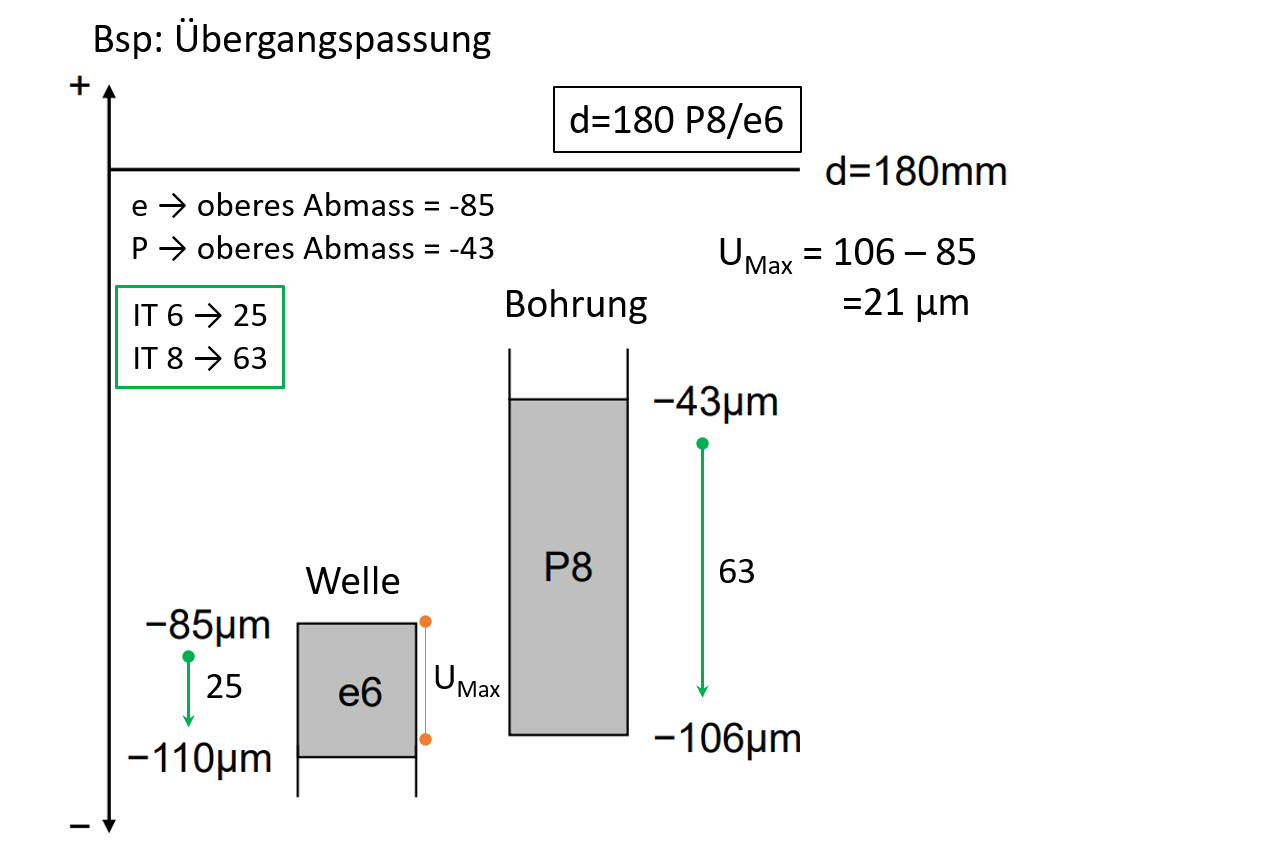
\includegraphics[width = 0.9\linewidth]{src/images/Passungen_bsp.png}
